\chapter{Neurones, potentiels d'action et synapses}\label{ch:b2:neurons-synapses}

Frappez le tendon sous la rotule, et la jambe se détend trente
millisecondes plus tard. Dans ce laps de temps, un étirement a été perçu
dans la cuisse, un signal a parcouru un mètre jusqu'à la moelle
épinière, a franchi une jonction vers une deuxième cellule, a parcouru
un mètre en sens inverse et a déclenché la contraction d'un muscle ---
l'aller-retour entier plus rapide qu'un clignement d'œil. Aucune
\omterm{def:b2:cell-signalling:kinds}{hormone} n'en serait capable~; cela est l'œuvre de cellules construites
pour conduire, et d'un signal qui n'est pas une substance en mouvement
mais une onde électrique régénérée le long d'une membrane. Ce chapitre
traite de cette cellule et de ce signal~: la tension qu'un \omterm{def:b2:neurons-synapses:neuron}{neurone}
maintient de part et d'autre de sa membrane, l'influx qu'il émet et la
manière dont cet influx se propage, et la \omterm{def:b2:neurons-synapses:synapse}{synapse}, où le signal
électrique est converti en signal chimique puis de nouveau en signal
électrique.

\section{Le neurone}

\begin{definition}[Neurone, axone, nerf]\label{def:b2:neurons-synapses:neuron}
\index{neurone}\index{axone}\index{dendrite}\index{myeline@myéline}\index{glie}
Un \emph{neurone} est une cellule spécialisée dans la signalisation~: un
corps cellulaire (\emph{soma}) qui contient le noyau, des
\emph{dendrites} ramifiées qui reçoivent les signaux, et un seul
\emph{axone} --- un câble d'un à vingt micromètres d'épaisseur et
jusqu'à un mètre de long --- qui porte le message de sortie jusqu'à des
\emph{terminaisons} au contact d'autres cellules. Le cerveau humain
compte quelque $10^{11}$ neurones, qui établissent chacun un millier de
\omterm{def:b2:neurons-synapses:synapse}{synapses} environ. Les neurones sont moins nombreux que les cellules de la
\emph{glie}~: les astrocytes, qui les nourrissent et tamponnent leur
milieu, les cellules microgliales, qui les surveillent, et les cellules
qui enroulent autour des axones la \emph{myéline} --- des dizaines de
tours de leur propre membrane, presque dépourvue de cytoplasme, formant
une gaine isolante interrompue environ tous les millimètres aux
\emph{\omterm{prop:b2:neurons-synapses:myelin}{nœuds de Ranvier}}. Un \emph{nerf} est un faisceau de milliers
d'axones, sensitifs et moteurs, qui cheminent ensemble dans un tissu
conjonctif. Les neurones ne se divisent pas chez l'adulte (à de rares
exceptions près), et un axone séparé de son corps cellulaire meurt~: un
neurone est une cellule qui doit durer toute une vie.
\end{definition}

\begin{omfigure}
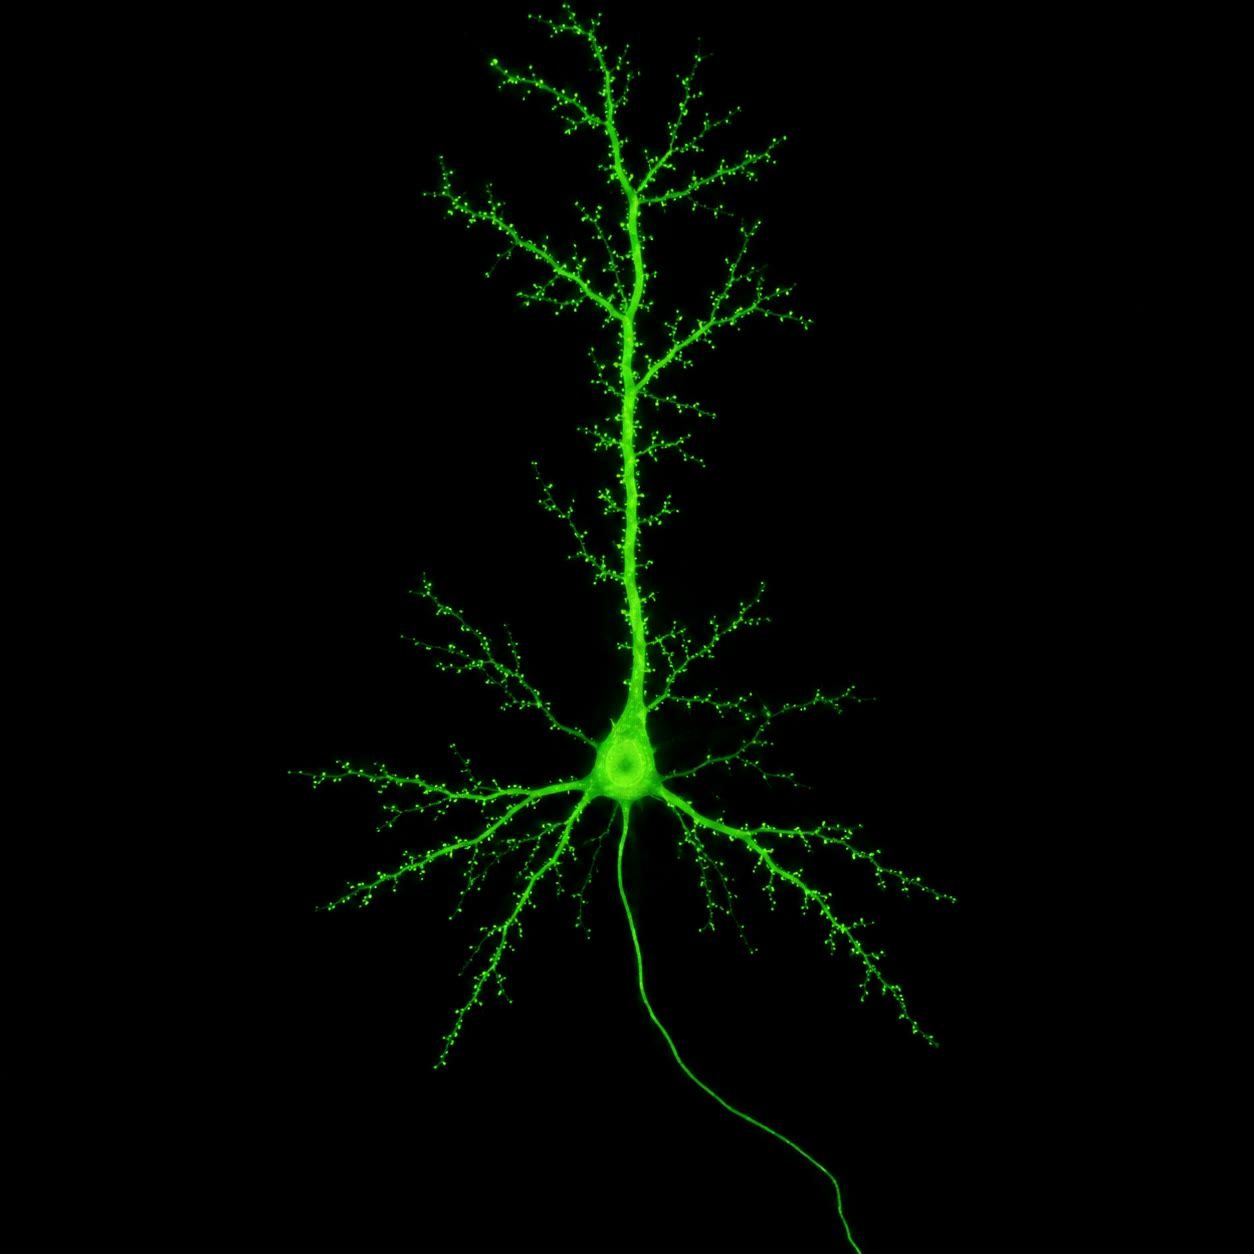
\includegraphics[width=0.4\linewidth]{images/book4/ai/b4-20-neuron-fluorescence.jpg}\hspace{0.05\linewidth}
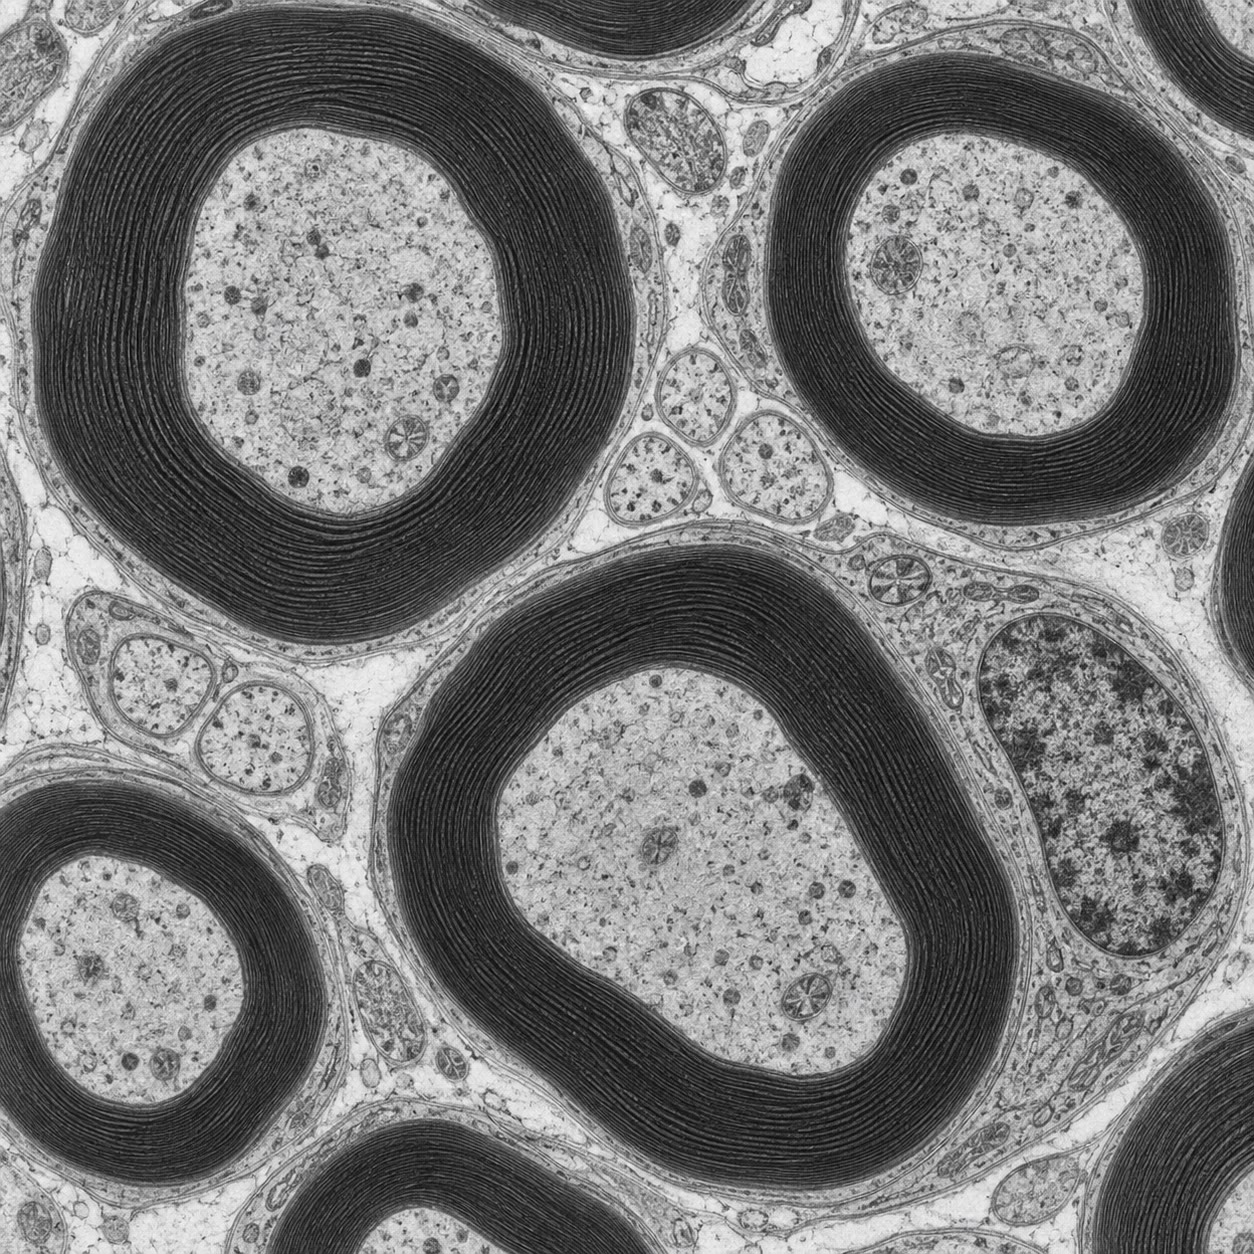
\includegraphics[width=0.4\linewidth]{images/book4/ai/b4-20-myelinated-axons-tem.jpg}

{\small À gauche~: un \omterm{def:b2:neurons-synapses:neuron}{neurone} pyramidal rempli de colorant --- le corps
cellulaire, les \omterm{def:b2:neurons-synapses:neuron}{dendrites} épineuses qui reçoivent, et le fin \omterm{def:b2:neurons-synapses:neuron}{axone} qui
part de sa base. À droite~: des \omterm{def:b2:neurons-synapses:neuron}{axones} en coupe transversale au
microscope électronique, chacun enveloppé dans la spirale sombre de sa
gaine de \omterm{def:b2:neurons-synapses:neuron}{myéline}.}
\end{omfigure}

\section{Le potentiel de repos}

\begin{theorem}[Le potentiel de Nernst]\label{thm:b2:neurons-synapses:nernst}
\index{potentiel de Nernst}\index{potentiel d'equilibre@potentiel d'équilibre}
Une membrane perméable à un seul ion de charge $z$, qui sépare des
concentrations $c_{\text{ext}}$ et $c_{\text{int}}$, se stabilise au
\emph{\omterm{thm:b2:neurons-synapses:nernst}{potentiel d'équilibre}}, pour lequel la force électrique qui
s'exerce sur l'ion équilibre sa diffusion~:
\[
E = \frac{RT}{zF}\ln\frac{c_{\text{ext}}}{c_{\text{int}}} \approx \frac{\qty{61.5}{mV}}{z}\log_{10}\frac{c_{\text{ext}}}{c_{\text{int}}} \quad (\qty{37}{\celsius}).
\]
Un \omterm{def:b2:neurons-synapses:neuron}{neurone} contient \qty{140}{mmol/L} de potassium à l'intérieur contre
\qty{5}{mmol/L} à l'extérieur, et \qty{15}{mmol/L} de sodium à
l'intérieur contre \qty{145}{mmol/L} à l'extérieur, des gradients
construits par la pompe sodium--potassium au prix d'un tiers de l'ATP
de la cellule. D'où $E_{\mathrm K} = 61.5\log_{10}(5/140) = \qty{-89}{mV}$ et
$E_{\mathrm{Na}} = 61.5\log_{10}(145/15) = \qty{+61}{mV}$~: si la
membrane ne laissait passer que le potassium, elle se placerait à
\qty{-89}{mV}, et si elle ne laissait passer que le sodium, à \qty{+61}{mV}.
\end{theorem}
\begin{proof}
À l'équilibre, le potentiel électrochimique de l'ion est le même
des deux côtés~: $RT\ln c_{\text{int}} + zFV_{\text{int}} = RT\ln
c_{\text{ext}} + zFV_{\text{ext}}$, donc $V_{\text{int}} -
V_{\text{ext}} = (RT/zF)\ln(c_{\text{ext}}/c_{\text{int}})$. À
\qty{310}{K}, $RT/F = \qty{26.7}{mV}$ et $\ln 10 \times 26.7 =
\qty{61.5}{mV}$. (Démontré dans le volume de première année à partir de
la distribution de Boltzmann~; rappelé ici.)
\end{proof}

\begin{theorem}[Le potentiel de repos, moyenne pondérée]\label{thm:b2:neurons-synapses:chord}
\index{potentiel de repos}\index{conductance (membrane)}
Si la membrane conduit plusieurs ions, chacun avec une conductance $g_i$
(la facilité avec laquelle elle le laisse passer, fixée par le nombre de
canaux ouverts), le potentiel stationnaire pour lequel les courants
s'annulent vaut
\[
V = \frac{\sum_i g_i E_i}{\sum_i g_i},
\]
une moyenne des \omterm{thm:b2:neurons-synapses:nernst}{potentiels d'équilibre} pondérée par les conductances.
Au repos, la membrane d'un \omterm{def:b2:neurons-synapses:neuron}{neurone} est environ vingt fois plus perméable
au potassium qu'au sodium, si bien que $V \approx (20\times(-89) +
61)/21 = \qty{-82}{mV}$~; en tenant compte du chlorure et des petites
fuites, le \omterm{thm:b2:neurons-synapses:chord}{potentiel de repos} vaut \qty{-70}{mV}. La membrane repose
près de $E_{\mathrm K}$ parce que des canaux potassiques sont ouverts~;
tout ce qui ouvre des canaux sodiques l'entraîne vers $E_{\mathrm{Na}}$
--- et c'est là tout le principe de la signalisation nerveuse.
\end{theorem}
\begin{proof}
Chaque ion porte un courant $I_i = g_i(V - E_i)$ (loi d'Ohm, la force
électromotrice étant mesurée à partir du \omterm{thm:b2:neurons-synapses:nernst}{potentiel d'équilibre} propre à
l'ion). À un potentiel stationnaire, le courant total est nul~: $\sum_i g_i(V - E_i) =
0$, d'où $V\sum g_i = \sum g_iE_i$. (Le traitement complet, dans lequel
les perméabilités interviennent par l'équation de Goldman--Hodgkin--Katz,
donne la même pondération au premier ordre.)
\end{proof}

\section{Le potentiel d'action}

\begin{proposition}[L'influx nerveux]\label{prop:b2:neurons-synapses:ap}
\index{potentiel d'action}\index{canal voltage-dependant@canal voltage-dépendant}\index{seuil}\index{periode refractaire@période réfractaire}
La membrane de l'\omterm{def:b2:neurons-synapses:neuron}{axone} porte des \emph{canaux sodiques voltage-dépendants},
fermés au repos et ouverts par la dépolarisation. Si un stimulus élève
le potentiel de \qty{-70}{mV} au-delà d'un \emph{seuil} voisin de
\qty{-55}{mV}, un nombre suffisant d'entre eux s'ouvrent pour laisser
entrer plus de sodium que la fuite de potassium ne peut en compenser~; le
potentiel monte, d'autres canaux s'ouvrent, et en une fraction de
milliseconde la membrane est entraînée vers
$E_{\mathrm{Na}}$ --- une \emph{rétroaction positive}, explosive
et en tout-ou-rien. Le potentiel culmine vers \qty{+40}{mV} parce que les
canaux sodiques \emph{s'inactivent} moins d'une milliseconde après leur
ouverture et parce que des \emph{canaux potassiques voltage-dépendants},
plus lents, s'ouvrent et ramènent le potentiel vers $E_{\mathrm K}$, en
le dépassant jusqu'à une \emph{hyperpolarisation} avant que les canaux
potassiques ne se referment. Le \emph{\omterm{prop:b2:neurons-synapses:ap}{potentiel d'action}} dure environ une
milliseconde~; pendant encore une ou deux millisecondes, les canaux
sodiques inactivés ne peuvent pas se rouvrir (la \emph{\omterm{prop:b2:neurons-synapses:ap}{période
réfractaire}}), ce qui limite la fréquence de décharge à quelques
centaines par seconde et oblige l'influx à se propager dans un seul
sens. Parce qu'il est en tout-ou-rien, l'influx ne porte aucune
information dans son amplitude~: le \omterm{def:b2:neurons-synapses:neuron}{neurone} code l'intensité par sa
\emph{fréquence}. Quelque
$10^{4}$ ions sodium entrent et autant d'ions potassium sortent à chaque
influx --- une variation de concentration négligeable, rétablie à loisir
par la pompe.
\end{proposition}
\begin{proof}[Faits expérimentaux]
Hodgkin et Huxley (1952), à l'aide de l'\omterm{def:b2:neurons-synapses:neuron}{axone} géant du calmar (épais
d'un demi-millimètre, si bien qu'on pouvait y introduire un fil) et d'un
amplificateur à rétroaction qui maintenait le potentiel de membrane à
n'importe quelle valeur choisie (le \emph{potentiel imposé}) tout en
enregistrant le courant nécessaire pour l'y maintenir, séparèrent ce
courant en une composante entrante précoce, qui disparaissait lorsqu'on
retirait le sodium du bain, et une composante sortante plus tardive,
portée par le potassium~; ils mesurèrent comment chaque conductance
augmentait puis diminuait au cours du temps à chaque tension~; et, en
ajustant chacune par quelques équations, ils calculèrent la forme, le
seuil, la vitesse et la \omterm{prop:b2:neurons-synapses:ap}{période réfractaire} du \omterm{prop:b2:neurons-synapses:ap}{potentiel d'action} à
partir des deux seules conductances. Toutes les prédictions se
vérifièrent. Les canaux eux-mêmes furent observés vingt-cinq ans plus
tard, un par un, avec la technique du patch-clamp~; la tétrodotoxine (le
poison du poisson-globe) bloque le canal sodique et abolit l'influx, le
tétraéthylammonium bloque le canal potassique et le prolonge.
\end{proof}

\begin{omfigure}
\begin{tikzpicture}
\begin{axis}[
  width=0.9\linewidth, height=6.4cm,
  axis x line=bottom, axis y line=left,
  xmin=0, xmax=4, ymin=-100, ymax=60,
  xlabel={temps (ms)}, ylabel={potentiel de membrane (mV)},
  xlabel style={font=\small, at={(axis description cs:0.5,-0.1)}, anchor=north},
  ylabel style={font=\small},
  tick label style={font=\small}, xtick={0,1,2,3,4}, ytick={-90,-70,-55,0,40},
  legend style={font=\scriptsize, at={(0.97,0.95)}, anchor=north east, draw=none},
  clip=false,
]
\addplot[very thick, omDef] coordinates {(0,-70) (0.4,-70) (0.5,-64) (0.6,-55) (0.7,-30) (0.8,10) (0.9,35) (1.0,40) (1.1,30) (1.2,10) (1.35,-20) (1.5,-50) (1.7,-75) (1.9,-85) (2.2,-82) (2.6,-76) (3.2,-71) (4,-70)};
\addlegendentry{potentiel de membrane}
\addplot[thick, omThm, dashed] coordinates {(0,0) (0.5,0) (0.6,5) (0.7,20) (0.8,35) (0.9,30) (1.0,20) (1.1,8) (1.2,3) (1.4,0) (4,0)};
\addlegendentry{$g_{\mathrm{Na}}$ (valeur relative)}
\addplot[thick, omProp, dashed] coordinates {(0,0) (0.6,0) (0.8,2) (1.0,8) (1.2,16) (1.4,20) (1.7,17) (2.0,10) (2.4,4) (3.0,1) (4,0)};
\addlegendentry{$g_{\mathrm K}$ (valeur relative)}
\draw[dashed, gray] (axis cs:0,-55) -- (axis cs:4,-55); \node[font=\scriptsize, anchor=south east] at (axis cs:4,-55) {seuil};
\draw[dashed, gray] (axis cs:0,-89) -- (axis cs:4,-89); \node[font=\scriptsize, anchor=south east] at (axis cs:3.7,-89) {$E_{\mathrm K}$};
\draw[<->, gray] (axis cs:1.0,50) -- (axis cs:2.5,50); \node[font=\scriptsize, anchor=south, gray] at (axis cs:1.75,50) {réfractaire};
\end{axis}
\end{tikzpicture}

{\small Un \omterm{prop:b2:neurons-synapses:ap}{potentiel d'action}. Au-delà du seuil, la conductance au sodium
(en rouge) augmente de façon explosive et entraîne le potentiel vers
$E_{\mathrm{Na}}$~; elle s'inactive tandis que la conductance au
potassium (en orange) augmente et ramène la membrane vers
$E_{\mathrm K}$, avec une hyperpolarisation. Sous la ligne du seuil, il ne
se passe rien.}
\end{omfigure}

\section{La conduction}

\begin{theorem}[Le câble et sa constante d'espace]\label{thm:b2:neurons-synapses:cable}
\index{constante d'espace}\index{equation du cable@équation du câble}\index{vitesse de conduction}
Un \omterm{def:b2:neurons-synapses:neuron}{axone} est un câble qui fuit~: un courant injecté en un point circule
dans le cytoplasme (résistance $r_i$ par unité de longueur) et fuit à
travers la membrane (résistance $r_m$ multipliée par l'unité de
longueur). Une dépolarisation constante $V_0$ en $x = 0$ décroît le long
de l'\omterm{def:b2:neurons-synapses:neuron}{axone} selon
\[
V(x) = V_0\,e^{-x/\lambda}, \qquad \lambda = \sqrt{\frac{r_m}{r_i}} = \sqrt{\frac{R_m\,d}{4R_i}},
\]
où $d$ est le diamètre et $R_m$, $R_i$ les résistances spécifiques de la
membrane et du cytoplasme. La \emph{\omterm{thm:b2:neurons-synapses:cable}{constante d'espace}}
$\lambda$ est la distance sur laquelle un signal passif tombe au
tiers~: environ \qty{0.5}{mm} pour un \omterm{def:b2:neurons-synapses:neuron}{axone} de \qty{1}{\micro m},
croissant comme la racine carrée du diamètre. Un \omterm{prop:b2:neurons-synapses:ap}{potentiel d'action} se
propage parce que la dépolarisation de son front, qui s'étend
passivement en avant sur environ $\lambda$, amène au seuil la portion
de membrane suivante, qui le régénère à pleine amplitude~; plus elle
porte loin, plus l'onde est rapide, si bien que la \omterm{thm:b2:neurons-synapses:cable}{vitesse de conduction}
croît elle aussi à peu près comme $\sqrt{d}$ --- de \qty{1}{m/s} dans une
fibre fine amyélinisée à \qty{20}{m/s} dans l'\omterm{def:b2:neurons-synapses:neuron}{axone} géant du calmar.
\end{theorem}
\begin{proof}
Soit $i(x)$ le courant axial et $V(x)$ la dépolarisation de la
membrane. La loi d'Ohm le long de l'axoplasme donne $\mathrm{d}V/
\mathrm{d}x = -r_i\,i$~; la conservation de la charge, avec la fuite à
travers la membrane, donne $\mathrm{d}i/\mathrm{d}x = -V/r_m$. En
combinant, $\mathrm{d}^{2}V/\mathrm{d}x^{2} = V/(r_m r_i)$, dont la
solution décroissante est $V_0 e^{-x/\lambda}$ avec $\lambda^{2} = r_m/r_i$. Pour un
cylindre, $r_m = R_m/(\pi d)$ et $r_i = 4R_i/(\pi d^{2})$, donc
$\lambda^{2} = R_m d/4R_i$. Avec $R_m = \qty{1}{\ohm.m^2}$, $R_i =
\qty{1}{\ohm.m}$ et $d = \qty{1}{\micro m}$~: $\lambda = \sqrt{10^{-6}
/4} = \qty{0.5}{mm}$.
\end{proof}

\begin{proposition}[Myéline et conduction saltatoire]\label{prop:b2:neurons-synapses:myelin}
\index{conduction saltatoire}\index{noeud de Ranvier@nœud de Ranvier}
La \omterm{def:b2:neurons-synapses:neuron}{myéline} multiplie $r_m$ par le nombre de tours de membrane et divise
la capacité de la membrane par le même facteur, si bien que sous la
gaine presque aucun courant ne fuit et qu'il faut peu de charge pour
modifier le potentiel~: la dépolarisation s'étend passivement le long
d'un internœud d'un millimètre avec peu de perte, et le \omterm{prop:b2:neurons-synapses:ap}{potentiel
d'action} n'est régénéré qu'aux nœuds, où les canaux sodiques sont
concentrés. L'influx \emph{saute} ainsi de nœud en nœud
(\emph{\omterm{prop:b2:neurons-synapses:myelin}{conduction saltatoire}}), à \qty{100}{m/s} dans une fibre de
\qty{20}{\micro m} --- une vitesse qu'un \omterm{def:b2:neurons-synapses:neuron}{axone} amyélinisé
n'atteindrait qu'avec une épaisseur de plusieurs centimètres --- et pour
une fraction du coût métabolique, puisque le sodium n'entre qu'aux
nœuds. La \omterm{def:b2:neurons-synapses:neuron}{myéline} est l'invention des vertébrés qui a rendu possible un
système nerveux vaste et rapide dans un petit corps~; dans la sclérose en
plaques, la gaine est détruite par plages, la \omterm{thm:b2:neurons-synapses:cable}{constante d'espace}
s'effondre et les influx échouent.
\end{proposition}

\begin{omfigure}
\begin{tikzpicture}[every node/.style={font=\scriptsize}, >=stealth]
  % unmyelinated
  \begin{scope}
    \draw[thick, fill=omDef!10] (0,0) rectangle (11,0.5);
    \foreach \x in {0.5,1.0,...,10.5} \draw[omThm, ->] (\x,0.25) -- (\x,0.9);
    \node[anchor=east] at (-0.2,0.25) {amyélinisé};
    \node[anchor=west] at (11.2,0.25) {\qty{1}{m/s}};
    \node[above] at (5.5,1.0) {l'influx est régénéré en chaque point};
  \end{scope}
  % myelinated
  \begin{scope}[yshift=-2.4cm]
    \draw[thick, fill=omDef!10] (0,0) rectangle (11,0.5);
    \foreach \x in {0.3,2.5,4.7,6.9,9.1} \fill[omExo!60] (\x,-0.15) rectangle (\x+1.9,0.65);
    \foreach \x in {2.35,4.55,6.75,8.95} \draw[omThm, ->] (\x,0.25) -- (\x,0.9);
    \foreach \x in {2.35,4.55,6.75} \draw[->, thick, omThm, dashed] (\x+0.1,1.1) .. controls (\x+1.1,1.6) .. (\x+2.1,1.1);
    \node[anchor=east] at (-0.2,0.25) {myélinisé};
    \node[anchor=west] at (11.2,0.25) {\qty{100}{m/s}};
    \node[below] at (1.25,-0.2) {internœud myélinisé};
    \node[below] at (4.55,-0.2) {nœud de Ranvier};
    \node[above] at (5.5,1.6) {régénéré seulement aux nœuds~: conduction saltatoire};
  \end{scope}
\end{tikzpicture}

{\small La conduction avec et sans \omterm{def:b2:neurons-synapses:neuron}{myéline}. Dans un \omterm{def:b2:neurons-synapses:neuron}{axone} nu, l'influx
est régénéré tout du long~; sous la \omterm{def:b2:neurons-synapses:neuron}{myéline}, le signal s'étend
passivement le long de chaque internœud et est régénéré aux nœuds, et
l'influx se propage cent fois plus vite.}
\end{omfigure}

\section{La synapse}

\begin{definition}[Synapses chimiques et électriques]\label{def:b2:neurons-synapses:synapse}
\index{synapse}\index{neurotransmetteur}\index{potentiel postsynaptique}
Au niveau d'une \emph{synapse}, la terminaison d'un \omterm{def:b2:neurons-synapses:neuron}{neurone} rencontre une
cible --- un autre \omterm{def:b2:neurons-synapses:neuron}{neurone}, une \omterm{def:b2:cell-differentiation:myogenesis}{fibre musculaire}, une cellule
glandulaire. Dans une synapse \emph{électrique}, des jonctions
communicantes relient les deux cellules et le courant passe directement
--- rapide, bidirectionnelle, sans amplification, utilisée là où
comptent la vitesse et la synchronie (réflexes de fuite, \omterm{def:b2:heart:anatomy}{cœur}). Dans une
synapse \emph{chimique}, les cellules sont séparées par une fente de
\qty{20}{nm} et le signal est une molécule. Un \omterm{prop:b2:neurons-synapses:ap}{potentiel d'action} qui
arrive à la terminaison ouvre des canaux calciques voltage-dépendants~;
le calcium entre et, en une fraction de milliseconde, fait fusionner
avec la membrane des vésicules de \emph{neurotransmetteur}, qui se
vident dans la fente~; le neurotransmetteur la traverse par diffusion en
quelques microsecondes et se fixe sur des récepteurs de la membrane
postsynaptique --- soit des canaux ioniques qu'il ouvre
(\emph{ionotropes}, rapides), soit des \omterm{prop:b2:cell-signalling:gpcr}{récepteurs couplés aux protéines G}
(\emph{métabotropes}, plus lents, \cref{ch:b2:cell-signalling})~; le
courant qui en résulte déplace le potentiel postsynaptique de quelques
millivolts, vers le haut (un \emph{potentiel postsynaptique excitateur},
dû à des canaux qui laissent passer le sodium) ou vers le bas (un
potentiel postsynaptique \emph{inhibiteur}, dû à des canaux qui laissent
passer le chlorure ou le potassium)~; et le neurotransmetteur est éliminé
en quelques millisecondes par une enzyme ou un transporteur. Le délai
est d'une demi-milliseconde~; ce prix achète la transmission à sens
unique, l'amplification, l'inhibition et la modifiabilité --- tout ce
dont un système nerveux a besoin au-delà de la simple conduction.
\end{definition}

\begin{omfigure}
\begin{tikzpicture}[every node/.style={font=\scriptsize}, >=stealth]
  % presynaptic terminal
  \draw[thick, fill=omDef!10] (0,0) .. controls (0,2.6) and (3.6,2.6) .. (3.6,0.2) -- (3.6,-0.2) .. controls (3.6,-2.6) and (0,-2.6) .. (0,0);
  \draw[very thick, omDef] (-2.2,0) -- (0.1,0); \node[omDef, above] at (-1.1,0.05) {axone};
  \foreach \p in {(2.0,1.0),(2.6,0.5),(2.7,-0.4),(2.1,-1.0),(1.6,0.2)} \draw[thick, fill=omProp!40] \p circle (0.25);
  \draw[thick, fill=omProp!40] (3.3,0.1) arc (90:-90:0.25) -- cycle;
  \foreach \p in {(3.75,0.2),(3.85,-0.1),(3.7,-0.35),(3.9,0.4)} \fill[omProp] \p circle (0.05);
  \fill[omThm] (3.45,1.3) circle (0.06); \node[omThm, anchor=east] at (3.35,1.45) {entrée de Ca$^{2+}$};
  \draw[->, omThm] (3.9,1.5) -- (3.55,1.35);
  % cleft
  \node[align=center, anchor=north] at (3.85,-2.75) {fente\\\qty{20}{nm}};
  \draw[gray] (3.85,-2.7) -- (3.85,-1.2);
  % postsynaptic
  \draw[thick, fill=omExo!15] (4.1,-2.6) rectangle (8.2,2.6);
  \foreach \y in {0.9,0.3,-0.3,-0.9} \draw[thick, fill=omDef!40] (4.05,\y-0.15) rectangle (4.45,\y+0.15);
  \node[anchor=west, align=left] at (4.6,0.3) {récepteurs~: les canaux\\s'ouvrent, les ions\\passent~: potentiel\\postsynaptique};
  \node[anchor=west, align=left] at (4.6,-1.7) {neurotransmetteur\\éliminé par une enzyme\\ou un transporteur};
  \node[anchor=west] at (4.6,2.2) {cellule postsynaptique};
  % labels
  \node[align=center, anchor=north] at (1.8,-2.75) {vésicules de\\neurotransmetteur};
  \node[anchor=south] at (1.8,2.75) {terminaison présynaptique};
\end{tikzpicture}

{\small Une \omterm{def:b2:neurons-synapses:synapse}{synapse} chimique. L'influx fait entrer du calcium, les
vésicules fusionnent et libèrent le \omterm{def:b2:neurons-synapses:synapse}{neurotransmetteur} dans la fente, les
récepteurs de la cible ouvrent des canaux, et le \omterm{def:b2:neurons-synapses:synapse}{neurotransmetteur} est
éliminé en quelques millisecondes.}
\end{omfigure}

\begin{theorem}[La libération quantique]\label{thm:b2:neurons-synapses:quantal}
\index{liberation quantique@libération quantique}\index{potentiel miniature}
Le \omterm{def:b2:neurons-synapses:synapse}{neurotransmetteur} est libéré par paquets --- des \emph{quanta},
une vésicule chacun --- et le nombre $k$ libéré par un influx est une
variable aléatoire. Si la terminaison possède $n$ sites de libération,
libérant chacun avec la probabilité $p$, et si $p$ est petite, $k$ suit
approximativement une loi de Poisson de moyenne $m = np$~:
\[
P(k) = \frac{m^{k}e^{-m}}{k!}, \qquad P(0) = e^{-m}, \qquad
m = \ln\frac{\text{nombre d'essais}}{\text{nombre d'échecs}}.
\]
Le contenu quantique moyen $m$ peut donc se lire sur la fraction des
influx qui ne libèrent rien, et se vérifier par la réponse moyenne
divisée par la taille d'un quantum. À une \omterm{prop:b2:neurons-synapses:integration}{jonction neuromusculaire}, $m$
vaut quelques centaines --- la transmission n'échoue jamais~; à une
\omterm{def:b2:neurons-synapses:synapse}{synapse} centrale, il est souvent voisin de un, et la \omterm{def:b2:neurons-synapses:synapse}{synapse} ne transmet
qu'une fraction des influx.
\end{theorem}
\begin{proof}
Avec $n$ sites indépendants libérant chacun avec la probabilité $p$, $k$
suit une loi binomiale~; pour $n$ grand et $p$ petit avec $np = m$ fixé,
la loi binomiale tend vers la loi de Poisson (la série de mathématiques,
deuxième année). $P(0) = e^{-m}$ donne $m$ à partir des échecs. La
vérification de Katz est que le même $m$, porté dans la formule de
Poisson, prédit les fractions observées de réponses à un, deux et trois
quanta.
\end{proof}
\begin{proof}[Faits expérimentaux]
Fatt et Katz (1952) enregistrèrent dans une \omterm{def:b2:cell-differentiation:myogenesis}{fibre musculaire} de
grenouille au repos de petites dépolarisations spontanées d'environ
\qty{0.5}{mV}, toutes de même taille, à intervalles aléatoires --- les
\emph{potentiels de plaque motrice miniatures}, chacun l'effet d'une
vésicule. Abaisser le calcium du bain réduisait la réponse à la
stimulation du nerf jusqu'à ce qu'elle fluctue entre 0, 1, 2 ou 3 fois la
taille miniature~; les fréquences de ces multiples suivaient la loi de
Poisson avec le
$m$ calculé à partir des échecs. Del Castillo et Katz montrèrent ainsi
que la libération est quantique, que le calcium contrôle la probabilité
de libération et non la taille d'un quantum, et la microscopie
électronique montra les vésicules qui constituent les quanta.
\end{proof}

\begin{proposition}[L'intégration~: le neurone comme décision]\label{prop:b2:neurons-synapses:integration}
\index{sommation}\index{cone d'emergence@cône d'émergence}\index{jonction neuromusculaire}
Un \omterm{def:b2:neurons-synapses:neuron}{neurone} central reçoit des milliers de \omterm{def:b2:neurons-synapses:synapse}{synapses}, excitatrices et
inhibitrices, sur ses \omterm{def:b2:neurons-synapses:neuron}{dendrites} et son soma. Chaque \omterm{def:b2:neurons-synapses:synapse}{potentiel
postsynaptique} est petit et décroît passivement, avec la \omterm{thm:b2:neurons-synapses:cable}{constante
d'espace} du câble dans l'espace et la constante de temps de la membrane
(quelques millisecondes) dans le temps~; ces potentiels s'additionnent
--- \emph{sommation spatiale} d'entrées qui arrivent ensemble,
\emph{sommation temporelle} d'entrées qui arrivent en succession rapide
--- et la somme est lue au \emph{\omterm{prop:b2:neurons-synapses:integration}{cône d'émergence}} de l'\omterm{def:b2:neurons-synapses:neuron}{axone}, où les
canaux sodiques sont les plus denses et le seuil le plus bas. Si la
somme franchit le seuil, l'\omterm{def:b2:neurons-synapses:neuron}{axone} décharge, à une fréquence qui croît avec
l'excès~; les entrées inhibitrices se soustraient, et une \omterm{def:b2:neurons-synapses:synapse}{synapse}
inhibitrice proche du \omterm{prop:b2:neurons-synapses:integration}{cône d'émergence} peut opposer son veto à une
\omterm{def:b2:neurons-synapses:synapse}{synapse} excitatrice éloignée. La
\omterm{prop:b2:neurons-synapses:integration}{jonction neuromusculaire} est l'exception qui confirme la règle~: une
seule terminaison motrice, libérant des centaines de quanta
d'acétylcholine sur des récepteurs qui sont aussi les canaux, produit un
potentiel de plaque motrice de \qty{50}{mV}, bien au-dessus du seuil ---
chaque influx du nerf moteur produit un \omterm{prop:b2:neurons-synapses:ap}{potentiel d'action} musculaire
(\cref{ch:b2:muscle-movement}). Le curare, qui bloque le récepteur,
paralyse~; les gaz neurotoxiques, qui bloquent l'enzyme qui élimine
l'acétylcholine, paralysent par l'excès inverse.
\end{proposition}

\begin{example}[Neurotransmetteurs et drogues]\label{ex:b2:neurons-synapses:transmitters}
L'acétylcholine à la \omterm{prop:b2:neurons-synapses:integration}{jonction neuromusculaire} et dans le \omterm{def:b2:blood-pressure:baroreflex}{système
nerveux autonome}~; le glutamate, principal \omterm{def:b2:neurons-synapses:synapse}{neurotransmetteur} excitateur
du cerveau, et le GABA, principal \omterm{def:b2:neurons-synapses:synapse}{neurotransmetteur} inhibiteur~; les
monoamines --- noradrénaline, dopamine et sérotonine ---, qui modulent
des circuits entiers à partir de quelques milliers de cellules~; et des
dizaines de peptides. Presque toutes les drogues et tous les médicaments
qui agissent sur le psychisme agissent sur une \omterm{def:b2:neurons-synapses:synapse}{synapse}~: les
benzodiazépines renforcent le canal du GABA, les antidépresseurs bloquent
le transporteur de la sérotonine, la cocaïne celui de la dopamine, les
opiacés imitent un peptide, la nicotine imite l'acétylcholine sur un
récepteur et l'atropine la bloque sur un autre, la toxine botulique
coupe les protéines qui font fusionner la vésicule. La \omterm{def:b2:neurons-synapses:synapse}{synapse} est le
lieu où la chimie du \cref{ch:b2:cell-signalling} et l'électricité de
ce chapitre se rencontrent, et où un système nerveux apprend~: les
\omterm{def:b2:neurons-synapses:synapse}{synapses} utilisées se renforcent, et ce renforcement (le volume de
troisième année) est la mémoire.
\end{example}

\section{Exercices}

\begin{exercise}[$\star$]\label{exo:b2:neurons-synapses:1}
Nommer les parties d'un \omterm{def:b2:neurons-synapses:neuron}{neurone} et la fonction de chacune, et dire de
quoi est faite la \omterm{def:b2:neurons-synapses:neuron}{myéline} et quel est son rôle.
\end{exercise}

\begin{exercise}[$\star$]\label{exo:b2:neurons-synapses:2}
Décrire les phases d'un \omterm{prop:b2:neurons-synapses:ap}{potentiel d'action} et les événements des canaux
qui provoquent chacune d'elles. Pourquoi est-il en tout-ou-rien, et
pourquoi ne se propage-t-il pas en sens inverse~?
\end{exercise}

\begin{exercise}[$\star$]\label{exo:b2:neurons-synapses:3}
Énumérer les étapes de la transmission à une \omterm{def:b2:neurons-synapses:synapse}{synapse} chimique, de
l'arrivée de l'influx à l'élimination du \omterm{def:b2:neurons-synapses:synapse}{neurotransmetteur}.
\end{exercise}

\begin{exercise}[$\star$]\label{exo:b2:neurons-synapses:4}
Comparer \omterm{def:b2:neurons-synapses:synapse}{synapses} électriques et chimiques du point de vue de la
vitesse, du sens de transmission, de l'amplification et de la
possibilité d'inhibition.
\end{exercise}

\begin{exercise}[$\star\star$]\label{exo:b2:neurons-synapses:5}
Calculer les \omterm{thm:b2:neurons-synapses:nernst}{potentiels de Nernst} à \qty{37}{\celsius} du potassium
(140 à l'intérieur, 5 à l'extérieur), du sodium (15 à l'intérieur,
145 à l'extérieur), du chlorure (10 à l'intérieur, 110 à l'extérieur)
et du calcium (\qty{1e-4}{} à l'intérieur, 2 à l'extérieur, en
\unit{mmol/L}). Dans quel sens chaque ion circule-t-il lorsque la
membrane est à \qty{-70}{mV}~?
\end{exercise}

\begin{exercise}[$\star\star$]\label{exo:b2:neurons-synapses:6}
Avec $E_{\mathrm K} = \qty{-89}{mV}$ et $E_{\mathrm{Na}} =
\qty{+61}{mV}$, calculer le potentiel de membrane lorsque $g_{\mathrm K} :
g_{\mathrm{Na}} = 20 : 1$ (repos), $1 : 20$ (sommet de l'influx)
et $50 : 1$ (hyperpolarisation). Expliquer chaque état.
\end{exercise}

\begin{exercise}[$\star\star$]\label{exo:b2:neurons-synapses:7}
Dans les \omterm{def:b2:neurons-synapses:neuron}{axones} amyélinisés, la \omterm{thm:b2:neurons-synapses:cable}{vitesse de conduction} varie comme $\sqrt d$, avec
\qty{1}{m/s} pour \qty{1}{\micro m}. Calculer la vitesse d'un \omterm{def:b2:neurons-synapses:neuron}{axone} de
calmar de \qty{0.5}{mm}. Une fibre myélinisée de \qty{20}{\micro m}
conduit à \qty{100}{m/s}~: quelle épaisseur devrait avoir un \omterm{def:b2:neurons-synapses:neuron}{axone}
amyélinisé pour l'égaler~? Combien de temps met un influx pour aller de
la moelle épinière à l'orteil (\qty{1}{m}) dans chaque fibre~?
\end{exercise}

\begin{exercise}[$\star\star$]\label{exo:b2:neurons-synapses:8}
Sur 200 stimulations d'une \omterm{def:b2:neurons-synapses:synapse}{synapse} dans un milieu pauvre en calcium, 74
ne produisent aucune réponse. Calculer le contenu quantique moyen et les
fractions prédites de réponses à un, deux et trois quanta. Le quantum
unitaire vaut \qty{0.5}{mV}~: quelle réponse moyenne attend-on~?
\end{exercise}

\begin{exercise}[$\star\star$]\label{exo:b2:neurons-synapses:9}
La \omterm{prop:b2:neurons-synapses:ap}{période réfractaire} d'un \omterm{def:b2:neurons-synapses:neuron}{neurone} est de \qty{2}{ms}. Quelle est sa
fréquence de décharge maximale~? Un \omterm{def:b2:neurons-synapses:neuron}{neurone} sensitif décharge à 20
influx par seconde pour un toucher léger et à 200 pour un toucher appuyé~:
qu'est-ce qui est codé, et par quoi~?
\end{exercise}

\begin{exercise}[$\star\star\star$]\label{exo:b2:neurons-synapses:10}
Calculer la \omterm{thm:b2:neurons-synapses:cable}{constante d'espace} pour $R_m = \qty{1}{\ohm.m^2}$, $R_i =
\qty{1}{\ohm.m}$ et des diamètres de 1, 10 et \qty{500}{\micro m}. La
\omterm{def:b2:neurons-synapses:neuron}{myéline} multiplie $R_m$ par 200~: refaire le calcul pour \qty{10}{\micro m}.
Expliquer pourquoi un internœud de \qty{1}{mm} fonctionne et pourquoi
une portion démyélinisée de \qty{3}{mm} bloque l'influx.
\end{exercise}

\begin{exercise}[$\star\star\star$]\label{exo:b2:neurons-synapses:11}
Prévoir l'effet sur le \omterm{prop:b2:neurons-synapses:ap}{potentiel d'action} et sur la transmission à la
\omterm{prop:b2:neurons-synapses:integration}{jonction neuromusculaire}~: de la tétrodotoxine~; du
tétraéthylammonium~; d'un bain sans calcium~; du curare~; d'un
inhibiteur de l'acétylcholinestérase~; de la toxine botulique.
\end{exercise}

\begin{exercise}[$\star\star\star$]\label{exo:b2:neurons-synapses:12}
«~Une \omterm{def:b2:neurons-synapses:synapse}{synapse} chimique coûte une demi-milliseconde et achète un système
nerveux.~» Discuter ce que paie ce délai --- transmission à sens unique,
amplification, inhibition, plasticité --- et dire où l'organisme utilise
à la place des \omterm{def:b2:neurons-synapses:synapse}{synapses} électriques.
\end{exercise}

\section{Problème~: le réflexe rotulien chronométré}

\begin{problem}[{Problème du week-end --- le réflexe myotatique suivi de
la percussion du tendon jusqu'à la détente de la jambe, avec le calcul
du potentiel de repos du neurone, la chronologie de la conduction de
l'influx le long des deux branches de l'arc, la mesure du contenu
quantique de la synapse, et le bilan de la latence entière, jusqu'au
potentiel de repos, aux temps de conduction, au contenu quantique et à
la latence du réflexe}]
\label{pb:b2:neurons-synapses:1}
Données à \qty{37}{\celsius}~: potassium, 140 à l'intérieur, 4 à
l'extérieur~; sodium, 12 à l'intérieur,
145 à l'extérieur (\unit{mmol/L})~; $g_{\mathrm K} : g_{\mathrm{Na}} = 25 : 1$
au repos. \omterm{def:b2:neurons-synapses:neuron}{Axones} sensitifs et moteurs~: \qty{15}{\micro m}, myélinisés,
\qty{90}{m/s}, \qty{0.9}{m} dans chaque sens. Délai synaptique \qty{0.6}{ms}~;
activation du muscle après son propre \omterm{prop:b2:neurons-synapses:ap}{potentiel d'action} \qty{5}{ms}.
\omterm{def:b2:neurons-synapses:synapse}{Synapse} centrale dans un milieu pauvre en calcium~: 300 essais, 111
échecs. Quantum \qty{0.4}{mV}~; seuil \qty{15}{mV} au-dessus du repos. $R_m =
\qty{1}{\ohm.m^2}$, $R_i = \qty{1}{\ohm.m}$~; la \omterm{def:b2:neurons-synapses:neuron}{myéline} multiplie $R_m$
par 250.

\medskip
\noindent\textbf{Partie I --- Le \omterm{def:b2:neurons-synapses:neuron}{neurone} au repos.}
\begin{enumerate}
  \item Calculer $E_{\mathrm K}$ et $E_{\mathrm{Na}}$.
  \item Calculer le \omterm{thm:b2:neurons-synapses:chord}{potentiel de repos} à partir du rapport des conductances.
  \item Le potassium extracellulaire monte à \qty{8}{mmol/L} (comme
        après un exercice intense). Recalculer $E_{\mathrm K}$ et le
        \omterm{thm:b2:neurons-synapses:chord}{potentiel de repos}, et dire l'effet sur l'excitabilité.
  \item La pompe s'arrête. Expliquer ce que deviennent les gradients et
        le potentiel en quelques heures, et pourquoi la cellule gonfle.
  \item Combien d'ions sodium entrent dans un \omterm{def:b2:neurons-synapses:neuron}{axone} de \qty{15}{\micro m}
        par millimètre et par influx si la capacité de la membrane vaut
        \qty{0.01}{F/m^2} et que le potentiel varie de \qty{100}{mV}~?
        ($Q = CV$~; un ion porte \qty{1.6e-19}{C}.)
  \item De quelle fraction cela modifie-t-il la concentration interne
        de sodium (volume de l'\omterm{def:b2:neurons-synapses:neuron}{axone} par millimètre)~?
  \item La pompe exporte trois ions sodium par ATP. Combien d'ATP
        coûte le retour à l'état initial après un influx, par millimètre d'\omterm{def:b2:neurons-synapses:neuron}{axone}~?
\end{enumerate}

\medskip
\noindent\textbf{Partie II --- La conduction.}
\begin{enumerate}[resume]
  \item Calculer le temps que met l'influx sensitif pour atteindre la
        moelle épinière et l'influx moteur pour atteindre le muscle.
  \item Calculer la \omterm{thm:b2:neurons-synapses:cable}{constante d'espace} d'un \omterm{def:b2:neurons-synapses:neuron}{axone} nu de \qty{15}{\micro m}
        et du même \omterm{def:b2:neurons-synapses:neuron}{axone} sous la \omterm{def:b2:neurons-synapses:neuron}{myéline}.
  \item Un internœud mesure \qty{1.5}{mm}. Quelle fraction de la
        dépolarisation d'un nœud atteint passivement le nœud suivant, avec
        et sans \omterm{def:b2:neurons-synapses:neuron}{myéline}~? Dans quel cas le nœud suivant peut-il être amené
        au seuil (\qty{15}{mV} à partir d'un influx de \qty{100}{mV})~?
  \item Amyélinisé, le même \omterm{def:b2:neurons-synapses:neuron}{axone} conduirait à $\sqrt{15}$
        m/s. Calculer l'aller-retour et commenter.
  \item Une plage de \qty{4}{mm} perd sa \omterm{def:b2:neurons-synapses:neuron}{myéline}. Calculer la
        fraction du signal qui la franchit et dire si le réflexe
        persiste.
  \item Pourquoi la \omterm{prop:b2:neurons-synapses:ap}{période réfractaire} fait-elle se propager l'influx
        dans un seul sens le long de l'\omterm{def:b2:neurons-synapses:neuron}{axone} sensitif~?
\end{enumerate}

\medskip
\noindent\textbf{Partie III --- La \omterm{def:b2:neurons-synapses:synapse}{synapse}.}
\begin{enumerate}[resume]
  \item Calculer le contenu quantique moyen $m$ à partir des échecs.
  \item Calculer les fractions prédites de réponses à 1, 2 et 3
        quanta, et les nombres attendus sur les 300 essais.
  \item Calculer le \omterm{def:b2:neurons-synapses:synapse}{potentiel postsynaptique} moyen.
  \item En calcium normal, la même \omterm{def:b2:neurons-synapses:synapse}{synapse} a $m = 60$. Quelle est la
        probabilité d'un échec, et la réponse moyenne~? Une seule \omterm{def:b2:neurons-synapses:synapse}{synapse}
        de ce type fait-elle décharger le motoneurone~?
  \item Le motoneurone reçoit \num{20} \omterm{def:b2:neurons-synapses:synapse}{synapses} sensitives de ce type,
        actives simultanément. Expliquer comment elles se somment et si
        le seuil est atteint.
  \item Une \omterm{def:b2:neurons-synapses:synapse}{synapse} inhibitrice sur le même \omterm{def:b2:neurons-synapses:neuron}{neurone} ouvre des canaux
        chlorure ($E_{\mathrm{Cl}} = \qty{-70}{mV}$, le \omterm{thm:b2:neurons-synapses:chord}{potentiel
        de repos}). Expliquer comment elle peut réduire la réponse
        excitatrice sans hyperpolariser la cellule.
\end{enumerate}

\medskip
\noindent\textbf{Partie IV --- Le réflexe entier.}
\begin{enumerate}[resume]
  \item Additionner~: conduction sensitive, délai synaptique, conduction
        motrice, délai neuromusculaire (\qty{0.6}{ms}), activation du
        muscle. Comparer aux \qty{30}{ms} mesurées.
  \item D'où vient le reste de la latence mesurée~?
  \item Le réflexe comporte une seule \omterm{def:b2:neurons-synapses:synapse}{synapse} (il est monosynaptique).
        Expliquer pourquoi un réflexe de retrait, avec deux ou trois
        \omterm{def:b2:neurons-synapses:synapse}{synapses} dans la moelle, est plus lent mais plus souple.
  \item La même percussion chez une patiente atteinte de démyélinisation
        périphérique donne un réflexe en retard de \qty{60}{ms}. Estimer
        la \omterm{thm:b2:neurons-synapses:cable}{vitesse de conduction} dans ses nerfs.
  \item Une dose de tétrodotoxine bloque la moitié des canaux sodiques.
        Prévoir l'effet sur le seuil, l'influx et le réflexe.
  \item Énoncer le résultat~: le \omterm{thm:b2:neurons-synapses:chord}{potentiel de repos}, les temps de
        conduction sensitive et motrice, le contenu quantique $m$, et la
        latence calculée du réflexe.
\end{enumerate}
\end{problem}
